\documentclass[12pt, a4paper, oneside]{ctexart}
\usepackage{amsmath, amsthm, amssymb, bm, color, graphicx, geometry, mathrsfs,extarrows, braket, booktabs, array}
\usepackage[colorlinks,linkcolor=red,anchorcolor=blue,citecolor=blue,urlcolor=blue,menucolor=black]{hyperref}
%%%% 设置中文字体 %%%%
\setCJKmainfont{方正新书宋_GBK.ttf}[ BoldFont = 方正小标宋_GBK, ItalicFont = 方正楷体_GBK]
%%%% 设置英文字体 %%%%
\setmainfont{Times New Roman}
\setsansfont{Calibri}
\setmonofont{Consolas}

\linespread{1.4}
%\geometry{left=2.54cm,right=2.54cm,top=3.18cm,bottom=3.18cm}
\geometry{left=1.84cm,right=1.84cm,top=2.18cm,bottom=2.18cm}
\newcounter{problem}  % 问题序号计数器
\newenvironment{problem}{\stepcounter{problem}\par\noindent\textbf{题目\arabic{problem}. }}{\smallskip\par}
\newenvironment{solution}[1]{\par\noindent\textbf{#1解答. }}{\smallskip\par}
\newenvironment{note}{\par\noindent\textbf{注记. }}{\smallskip\par}

\usepackage{minted}
\renewcommand{\theFancyVerbLine}{
    \sffamily\textcolor[rgb]{0.5,0.5,0.5}{\scriptsize\arabic{FancyVerbLine}}} % 修改代码前序号大小
\newmintinline{python}{linenos, breaklines, frame=lines, python3}  % 使用\pythoninline{代码}
\newmintinline{cpp}{linenos, breaklines, frame=lines}  % 使用\c++inline{代码}
\newminted{python}{linenos, breaklines, frame=lines, python3}  % 使用\begin{pythoncode}代码\end{pythoncode}
\newminted{cpp}{fontsize=\small, linenos, breaklines, frame=lines}  % 使用\begin{pythoncode}代码\end{pythoncode}
\newmintedfile{python}{linenos, breaklines, frame=lines, python3}  % 使用\pythonfile{代码地址}

%%%% 图片相对路径 %%%%
\graphicspath{{figure/}} % 当前目录下的figure文件夹, {../figure/}则是父目录的figure文件夹

\everymath{\displaystyle} % 默认全部行间公式
\DeclareMathOperator*\uplim{\overline{lim}} % 定义上极限 \uplim_{}
\DeclareMathOperator*\lowlim{\underline{lim}} % 定义下极限 \lowlim_{}
\DeclareMathOperator*{\argmax}{arg\,max}  % 定义取最大值的参数 \argmax_{}
\DeclareMathOperator*{\argmin}{arg\,min}  % 定义取最小值的参数 \argmin_{}
\let\leq=\leqslant % 将全部leq变为leqslant
\let\geq=\geqslant % geq同理

%%%% 一些宏定义 %%%%
\def\bd{\boldsymbol}        % 加粗(向量) boldsymbol
\def\disp{\displaystyle}    % 使用行间公式 displaystyle(默认)
\def\tsty{\textstyle}       % 使用行内公式 textstyle
\def\sign{\text{sign}}      % sign function
\def\wtd{\widetilde}        % 宽波浪线 widetilde
\def\R{\mathbb{R}}          % Real number
\def\N{\mathbb{N}}          % Natural number
\def\Z{\mathbb{Z}}          % Integer number
\def\Q{\mathbb{Q}}          % Rational number
\def\C{\mathbb{C}}          % Complex number
\def\d{\mathrm{d}}          % differential operator
\def\e{\mathrm{e}}          % Euler's number
\def\i{\mathrm{i}}          % imaginary number
\def\re{\mathrm{Re}}        % Real part
\def\im{\mathrm{Im}}        % Imaginary part
\def\res{\mathrm{Res}}      % Residue
\def\L{\mathcal{L}}         % Loss function
\def\O{\mathcal{O}}         % 时间复杂度
\def\wdh{\widehat}          % 宽帽子 widehat
\def\ol{\overline}          % 上横线 overline
\def\ul{\underline}         % 下横线 underline
\def\add{\vspace{1ex}}      % 增加行间距
\def\del{\vspace{-3.5ex}}   % 减少行间距

%%%% 定理类环境的定义 %%%%
\newtheorem{theorem}{定理}

%%%% 基本信息 %%%%
\newcommand{\RQ}{\today} % 日期
\newcommand{\km}{算法设计与分析} % 科目
\newcommand{\bj}{强基数学002} % 班级
\newcommand{\xm}{吴天阳} % 姓名
\newcommand{\xh}{2204210460} % 学号

\begin{document}

%\pagestyle{empty}
\pagestyle{plain}
\vspace*{-15ex}
\centerline{\begin{tabular}{*5{c}}
    \parbox[t]{0.25\linewidth}{\begin{center}\textbf{日期}\\ \large \textcolor{blue}{\RQ}\end{center}} 
    & \parbox[t]{0.25\linewidth}{\begin{center}\textbf{科目}\\ \large \textcolor{blue}{\km}\end{center}}
    & \parbox[t]{0.2\linewidth}{\begin{center}\textbf{班级}\\ \large \textcolor{blue}{\bj}\end{center}}
    & \parbox[t]{0.1\linewidth}{\begin{center}\textbf{姓名}\\ \large \textcolor{blue}{\xm}\end{center}}
    & \parbox[t]{0.15\linewidth}{\begin{center}\textbf{学号}\\ \large \textcolor{blue}{\xh}\end{center}} \\ \hline
\end{tabular}}
\begin{center}
    \zihao{3}\textbf{第三次作业}
\end{center}\vspace{-0.2cm}
% 正文部分
\begin{solution}{(3-1)}
    设序列数组为$a[n]$,长度为$n$,下标从$1$开始.

    \textbf{方法1(复杂度$\O(n^2)$)}:设$dp[i]$表示以$a[i]$结尾的前$a[1\cdots i]$中最长的单调递增子序列长度,$fa[i]$表示以$i$结尾的最长子序列的前一个下标位置. 初始化:$dp[0] = 0,\ a[0]=-\infty$. 则有以下转移方程
    \begin{equation*}
        dp[i] = \max_{\substack{0\leq j < i\\ a[j]\leq a[i]}}dp[j]+1,\ fa[i] = \argmax_{\substack{0\leq j < i\\ a[j] \leq a[i]}}dp[j].
    \end{equation*}
    则$m=\max_{1\leq i\leq n}dp[i]$为最长单调子序列的长度,设$k = \argmax_{1\leq i\leq n}dp[i]$,则$k$为最长子序列的结尾对应的下标,令$x_1 = fa[k], x_2 = fa[x_1], \cdots, x_{i+1} = fa[x_i],\cdots, x_{m+1} = 0$,则最长单调子序列为
    \begin{equation*}
        \{a[x_m], a[x_{m-1}], \cdots, a[x_1]\}.
    \end{equation*}

    \textbf{方法2(复杂度$\O(n\log n)$)}:考虑直接维护前$a[1\cdots i]$中的最长单调子序列,设$b$数组为前$i$个字符构成的最长单调子序列,令$b=\{a_{n_1},a_{n_2},\cdots,a_{n_k}\}$,满足$a_{n_1}\leq a_{n_2}\leq \cdots\leq a_{n_k}$,且满足$a_{n_i}$是对应为上最小值,即如果有多个相同长度的最长单调子序列,$a_{n_i}$一定是所有子序列第$i$位上的最小值.
    
    考虑第$i+1$个元素$a_{i+1}$,若$a_{i+1}\geq a_{n_k}$则在$b$的尾端加入$a_{i+1}$,否则在$b$中从左到右查找第一个大于$a_{i+1}$的位置$j$,由于$b$是单增的,所以可以通过二分查找加速,然后令$a_{n_j} = a_{i+1}$. 如此反复操作$n$次,即可得到整个数组的最长单调子序列$b$,且每个元素均为对应位上的最小元.
\end{solution}
\begin{solution}{(3-3)}
    设文章单词总共有$n$个,每个长度分别为$l_1,\cdots, l_n$,打印机每行最多打$M$个字符,不妨令$M\geq \argmax_{1\leq i\leq n}l_i$.\add
    
    设状态数组$dp[i][j]$表示第$i$行放$j$个单词的多余空格的最小立方和,初始化:$dp[0][0] = 0,\ dp[i][j] = +\infty, 1\leq i,j \leq n$,则转移方程为
    \begin{equation*}
        dp[i][j] = \min_{0\leq k < j}dp[i-1][k]+\left(M-\sum_{t=k+1}^jl_t-j+k+1\right)^3,\ fa[i][j] = \text{左式取到最小值时对应的}k\text{值}.
    \end{equation*}
    则$\min_{1\leq i\leq n}dp[i][n]$为最小代价,令$m = \argmin_{1\leq i\leq n}dp[i][n]$也就表示最小代价所需的行数. 则对单词下标$\{1,2,\cdots,n\}$按行得到的划分为
    \begin{equation*}
        a_m = n,\ a_{m-1} = fa[m][n],\ a_{m-2} = fa[m-1][a_{m-1}],\ \cdots,\ a_1=fa[2][a_2],\ a_0 = fa[1][a_1]=0.
    \end{equation*}
    第$i$行打印的单词为$\{l_j:j\in (a_{i-1}, a_i]\}$.
    
    总时空复杂度:$\O(n^2)$.
\end{solution}

% 下面给一些功能的写法
\iffalse
% 图片模板
\centerline{
    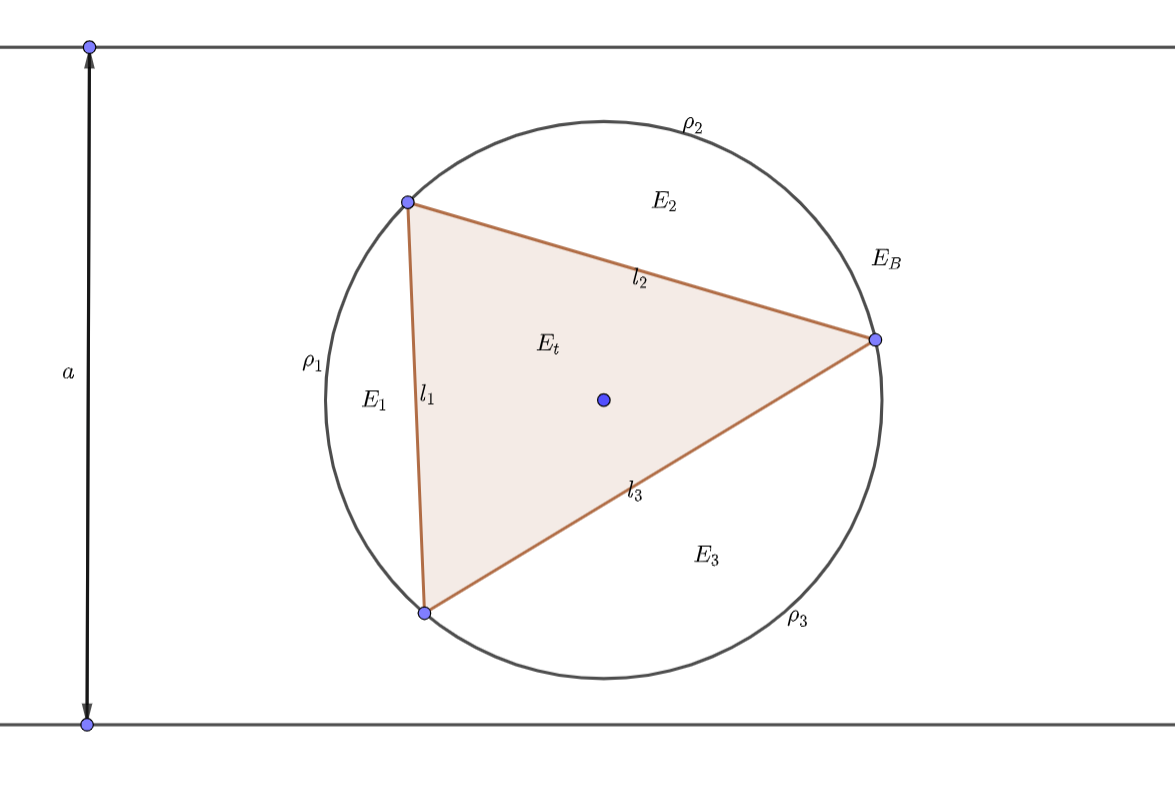
\includegraphics[width=0.8\textwidth]{figure.png}
}
% 表格模板
\renewcommand\arraystretch{0.8} % 设置表格高度为原来的0.8倍
\begin{table}[!htbp] % table标准
    \centering % 表格居中
    \begin{tabular}{p{1cm}<{\centering}p{1cm}<{\centering}p{3cm}<{\centering}p{5cm}<{\centering}} % 设置表格宽度
    %\begin{tabular}{cccc}
        \toprule
        $x_i$ & $f[x_1]$ & $f[x_i,x_{i+1}]$ & $f[x_i,x_{i+1},x_{i+2}]$ \\
        \midrule
        $x_0$ & $f(x_0)$ &                  &                          \\
        $x_0$ & $f(x_0)$ & $f'(x_0)$        &                          \\
        $x_0$ & $f(x_1)$ & $\frac{f(x_1)-f(x_0)}{x_1-x_0}$ & $\frac{f(x_1)-f(x_0)}{(x_1-x_0)^2}-\frac{f'(x_0)}{x_1-x_0}$\\
        \bottomrule
    \end{tabular}
\end{table}

\def\Log{\text{Log}} % 一个简单的宏定义
$\Log$ % 调用方法
\fi

\end{document}